% B.Tech Project report: A Simple Optimized SIP Strategy for Multi-Asset Allocation
% Build:  cd report && pdflatex main && bibtex main && pdflatex main && pdflatex main
\documentclass[11pt,a4paper]{article}

% ------------------------------------------------------------------ details to fill in
\newcommand{\studentname}{Mainak Biswas}
\newcommand{\rollno}{S20240030386}
\newcommand{\programme}{Bachelor of Technology (UG 3)}
\newcommand{\department}{Department of Artificial Intelligence and Data Science}
\newcommand{\college}{Indian Institute of Information Technology, Sri City}
\newcommand{\guide}{Dr.\ Mainak Thakur}
\newcommand{\submissiondate}{November 2026}
\newcommand{\reporttitle}{A Simple Optimized SIP Strategy for Multi-Asset Allocation Based on Back-Tested Data}

% ------------------------------------------------------------------ packages
\usepackage[T1]{fontenc}
\usepackage[utf8]{inputenc}
\usepackage{lmodern}
\usepackage[margin=1in]{geometry}
\usepackage{setspace}
\usepackage{amsmath,amssymb}
\usepackage{graphicx}
\usepackage{booktabs}
\usepackage{tabularx}
\usepackage{array}
\usepackage{float}
\usepackage[font=small,labelfont=bf]{caption}
\usepackage{xcolor}
\usepackage{listings}
\usepackage{tikz}
\usetikzlibrary{arrows.meta,positioning,shapes.geometric}
\usepackage[round,authoryear]{natbib}
\usepackage[hidelinks]{hyperref}
\usepackage{enumitem}
\usepackage{adjustbox}
\usepackage{nicefrac}

\setstretch{1.2}
\graphicspath{{../}{figures/}}
\setlist{itemsep=2pt,topsep=4pt}

\newcommand{\Rs}{Rs.\,}
\newcommand{\code}[1]{\texttt{#1}}

\definecolor{codebg}{RGB}{246,247,249}
\lstset{
  basicstyle=\ttfamily\small,
  backgroundcolor=\color{codebg},
  frame=single, rulecolor=\color{gray!40},
  breaklines=true, columns=fullflexible,
  keywordstyle=\color{blue!60!black}\bfseries,
  commentstyle=\color{gray}\itshape,
  showstringspaces=false, xleftmargin=4pt, xrightmargin=4pt
}

\begin{document}

% ================================================================== title page
\begin{titlepage}
  \thispagestyle{empty}
  \centering
  \vspace*{0.5cm}
  {\LARGE\bfseries \reporttitle\par}
  \vspace{1.2cm}
  {\large A B.Tech Project Report\par}
  \vspace{0.4cm}
  {submitted in partial fulfilment of the requirements for the degree of\par}
  {\large\bfseries \programme\par}
  \vspace{1.2cm}
  {by\par}
  \vspace{0.3cm}
  {\Large\bfseries \studentname\par}
  {\large Roll No.\ \rollno\par}
  \vspace{1.2cm}
  {under the guidance of\par}
  \vspace{0.3cm}
  {\Large\bfseries \guide\par}
  \vfill
  % \includegraphics[width=3cm]{figures/logo.png}\par\vspace{0.5cm}   % add the college logo here
  {\large \department\par}
  {\large\bfseries \college\par}
  \vspace{0.3cm}
  {\large \submissiondate\par}
\end{titlepage}


% ================================================================== abstract
\section*{Abstract}
A Systematic Investment Plan (SIP) invests a fixed amount every month. This project asks how an
Indian SIP investor should split each instalment between three assets: Nifty~50 equities, gold
and a liquid (money-market) fund, using only information available at the time and taking the
investor's own tolerance for risk into account.

A monthly back-testing engine was built and applied to rupee returns constructed from
Feb~2000 to Oct~2026. Every allocation is decided from a rolling 120-month window, so no future
data is ever used. Eight strategies were compared: fixed mixes (100\% equity, equal weights,
60/20/20), optimiser-based mixes (risk parity, maximum Sharpe ratio and their average), a
corrected optimiser that treats the liquid fund as cash, and a direct mean-variance utility
maximiser. Strategies were scored with the mean-variance utility
$U = \text{return above the liquid fund} - \tfrac{\lambda}{2}\sigma^2$, where $\lambda$ is the
investor's risk aversion.

All design choices were fixed on 2010--2019 and tested on 2020--2025, data that played no part in
building them. The corrected optimiser had the highest utility for every investor profile out of
sample (XIRR 20.3\%), while directly maximising utility did not win, which illustrates the
estimation-error problem of mean-variance optimisation. The final rule, the \emph{Personal SIP},
keeps a liquid ``safety cushion'' chosen by utility for each risk level (10\%, 30\% or 70\%) and
splits the rest between Nifty and gold by averaging risk parity and maximum Sharpe. Out of sample it
cut the worst fall for a conservative investor from $-12.2\%$ to $-3.4\%$, at the cost of lower
returns during the 2020--2025 gold boom. The rule was implemented as a public website that turns
an investor's risk level, monthly amount and current holdings into this month's purchases; its
results match the Python engine to within half a rupee.






\section{Introduction}
\label{ch:intro}

\subsection{Background}

A \emph{Systematic Investment Plan} (SIP) is the most common way Indian retail investors buy
mutual funds: a fixed amount, for example \Rs10{,}000, is invested on the same date every month.
Most SIPs go into a single equity fund. Equity has the highest long-run return of the
mainstream asset classes, but it also falls the hardest: the Nifty~50 lost about 24\% in 2011 and
about 28\% during the COVID-19 crash of March 2020 (Section~\ref{ch:results}).

Two other assets are easy for an Indian investor to hold through mutual funds and exchange-traded
funds. \emph{Gold}, bought in rupees, has historically moved largely independently of Indian equities
and often rises when the rupee falls \citep{baur2010}. A \emph{liquid fund} invests in very
short-term government and money-market paper; it earns roughly the 91-day Treasury-bill rate and
almost never falls in value. Holding all three should give a smoother ride than equity alone. The
question is \emph{how much} of each month's instalment should go into each.

\subsection{Problem statement}

\begin{quote}
\emph{Given a fixed monthly investment and the investor's tolerance for risk, how should each
instalment be split between Nifty~50 equities, gold and a liquid fund, using only the data that
would have been available at the time?}
\end{quote}

The answer must be usable by an ordinary investor every month, so the study ends not with a table
of back-test results but with a tool that gives this month's instruction.

\subsection{Objectives}

\begin{enumerate}
  \item Build a clean, verified table of monthly rupee returns for the three assets from
        Feb~2000 to the latest available month (Section~\ref{ch:data}).
  \item Build a monthly SIP simulation engine with realistic instalments, rebalancing and costs,
        in which every decision uses only past data (Section~\ref{ch:method}).
  \item Compare simple fixed mixes with optimiser-based strategies on 2010--2019, and test all of
        them, unchanged, on 2020--2025 (Section~\ref{ch:results}).
  \item Define one score that balances return against risk for a given investor, and use it to
        choose between approaches (Sections~\ref{sec:utility} and \ref{sec:res-utility}).
  \item Turn the final rule into a website that any investor can use each month
        (Section~\ref{ch:website}).
\end{enumerate}


\section{Literature Review}
\label{ch:lit}

This section summarises the work on which each part of the project rests, in the order in which
the ideas are used.

\subsection{Mean-variance portfolio theory}

\citet{markowitz1952} showed that an investor who cares about expected return and variance should
not judge an asset on its own, but by what it adds to the whole portfolio. Assets that do not
move together reduce risk when combined; this diversification effect is the reason for holding Nifty
and gold together (Section~\ref{sec:maxsharpe}).

\citet{tobin1958} added a risk-free asset and showed that the problem separates into two decisions:
(i) the mix of risky assets, which is the same for every investor, and (ii) how much to hold in the
risk-free asset, which depends on the investor's attitude to risk. This \emph{separation} is the
basis of the Personal SIP (Section~\ref{sec:personal}): the liquid fund plays the role of the
risk-free asset, its share is set by the investor's risk aversion, and the Nifty/gold split is
common to everyone.

\subsection{Risk-adjusted performance: the Sharpe ratio}

\citet{sharpe1966} proposed the reward-to-variability ratio, later called the Sharpe ratio: the
return in excess of a risk-free rate divided by volatility. \citet{sharpe1994} restated it and
stressed that the benchmark rate must be the investor's actual alternative. This point turned out
to be central in this project: with a liquid fund in the portfolio, measuring excess return against
0\% instead of against the liquid fund makes cash look nearly perfect
(Section~\ref{sec:res-2010}).

\subsection{Risk aversion and mean-variance utility}

\citet{pratt1964} formalised \emph{risk aversion} and the \emph{certainty equivalent}: the sure
amount an investor would accept in place of a risky prospect. For returns that are not extreme,
expected utility is closely approximated by a function of mean and variance alone, and
\citet{levy1979} and \citet{kroll1984} showed empirically that portfolios chosen by such a
mean-variance score are almost identical to those chosen by maximising expected utility directly.
The standard textbook form \citep{bkm2021} is
\begin{equation*}
  U = E(r) - \tfrac{1}{2}A\sigma^2 ,
\end{equation*}
where $A$ is the risk-aversion coefficient. This project uses the same form with returns measured
above the liquid fund and $A$ written as $\lambda$ (Section~\ref{sec:utility}). Maximising $U$ is
equivalent to Markowitz's problem of maximising return for a given variance, with $\lambda$ acting
as the Lagrange multiplier on the variance constraint.

\subsection{Risk parity}

Risk parity allocates so that each asset contributes the same share of total portfolio risk.
\citet{maillard2010} define the risk contribution of asset $i$ as $w_i(\Sigma w)_i$ and study the
equal-risk-contribution portfolio; \citet{qian2006} shows that these contributions add up to total
variance and can be read as each asset's share of likely losses. \citet{asness2012} explain why such
portfolios have historically delivered good risk-adjusted returns. Because risk parity uses only
volatilities and correlations, not expected returns, it is far less sensitive to estimation error,
which is why it is one of the two components of the allocation rule used here.

\subsection{Estimation error}

Optimisers need estimates of expected returns, variances and covariances, and these are noisy.
\citet{michaud1989} showed that mean-variance optimisers act as ``error maximisers'': they put the
most weight on assets whose returns happen to be overestimated. \citet{chopra1993} found that errors
in expected returns are roughly ten times as damaging as errors in variances. \citet{demiguel2009}
found that a simple $1/N$ (equal-weight) portfolio was not consistently beaten out of sample by
fourteen optimised models, while \citet{kritzman2010} argued that optimisation does add value when
inputs are estimated sensibly. This debate is tested directly in Section~\ref{ch:results}, where an
equal-weight SIP, several optimisers and a direct utility maximiser are compared on unseen data.
\citet{bailey2014} warn that trying many variations on one data set produces back-tests that look
good by chance; the strict separation of design (2010--2019) and test (2020--2025) periods in this
project follows that advice.

\subsection{Gold, SIPs and rebalancing}

Gold is a hedge against equities on average and a safe haven in market crashes \citep{baur2010}; for an Indian investor, rupee gold also rises when the rupee weakens. 
A SIP is a form of rupee-cost averaging, which is not optimal for a lump sum \citep{constantinides1979,vanduffel2012}; for a salaried investor with no lump sum, the question becomes how to allocate each instalment. How often to rebalance is studied by \citet{perold1988}, who compare constant-mix and other dynamic
strategies, and by \citet{jaconetti2010}, who recommend rebalancing only when allocations drift
beyond a threshold, in the range of about 5\%, rather than on a fixed calendar. The 5\% band rule in
this project's engine follows that recommendation.


\chapter{Data}
\label{ch:data}

Every strategy in this project reads one table: the monthly return, in rupees, of each of the three
assets. This chapter explains how that table was built for three periods with different sources,
and how each source was checked.

\section{The three assets}

\begin{table}[H]
\centering
\caption{The three assets}
\label{tab:assets}
\begin{tabularx}{\textwidth}{@{}lXX@{}}
\toprule
Asset & What it represents & Behaviour \\
\midrule
Nifty & India's 50 largest listed companies (Nifty~50), with dividends & Highest long-run return; large swings \\
Gold & Gold bought in Indian rupees & Swings, but often at different times from equities \\
Liquid & A liquid fund: very short-term government and money-market paper & Earns about the 91-day T-bill rate; almost never falls \\
\bottomrule
\end{tabularx}
\end{table}

\section{From prices to monthly returns}

A SIP invests once a month, so each daily series is sampled at the month end and turned into the
growth of one rupee over the month:
\begin{equation}
  r_t = \frac{P_t}{P_{t-1}} - 1 ,
  \label{eq:return}
\end{equation}
where $P_t$ is the last available value in month $t$. Because a return needs a previous month, the
closing values of January~2000 are the starting point and the first return is for February~2000.

\section{Period 1: Feb 2000 -- Dec 2019}

The base file contains daily values of the Nifty~50 price index, the international gold price in US
dollars per ounce, and a liquid-fund index that grows each day by the 91-day T-bill yield divided by
365. Three adjustments turn these into what an Indian investor actually earns.

\paragraph{Nifty dividends.} An index-fund investor also receives the companies' dividends, which
the price index excludes. A constant dividend yield of 1.3\% a year is added:
\begin{equation}
  r_{\text{Nifty},t} = \frac{P_t}{P_{t-1}} - 1 + \frac{0.013}{12}.
\end{equation}
For February 2010: $4{,}922.30 / 4{,}882.05 - 1 + 0.013/12 = 0.824\% + 0.108\% = 0.933\%$.
The Nifty dividend yield has historically been between 1\% and 2\%.

\paragraph{Gold in rupees.} An Indian investor pays for gold in rupees, so the dollar price is
converted with the USD/INR exchange rate \citep{fred}:
\begin{equation}
  G^{\text{INR}}_t = G^{\text{USD}}_t \times FX_t, \qquad
  r_{\text{Gold},t} = \frac{G^{\text{INR}}_t}{G^{\text{INR}}_{t-1}} - 1 .
\end{equation}
For February 2010: $\$1{,}118.9 \times 46.05 = \Rs51{,}525.35$ against $\$1{,}083.8 \times 46.08
= \Rs49{,}941.50$ in January, a return of $3.171\%$. Between 2000 and 2019 the rupee fell from about
43.5 to 71.4 per dollar, so rupee gold grew about 2.5\% a year faster than dollar gold.

\paragraph{Liquid.} The liquid index grows daily by the T-bill yield,
$L_d = L_{d-1}(1 + y_d/365)$, and its monthly return is computed with Eq.~\eqref{eq:return}. For
February 2010: $188.1263 / 187.5356 - 1 = 0.315\%$.

\paragraph{Verification.} Nifty closes were matched against two independent NSE-sourced files:
99.94\% of 4{,}812 trading days were identical, and the only differences were special weekend
sessions, none at a month end. The gold column was confirmed to be US dollars per ounce by matching a
monthly gold series \citep{worldbank} to within 0.33\% on average. The liquid index's implied rate
steps weekly, as 91-day T-bill auctions do, and follows the known history of Indian T-bill yields
(about 9.25\% in 2000, 3.3\% in 2009, a spike to 12\% in August 2013, 5--6\% in 2019).

\begin{table}[H]
\centering
\caption{Annual return and volatility of the three assets, Feb 2000 -- Dec 2019}
\label{tab:asset-stats}
\begin{adjustbox}{max width=\textwidth}
\begin{tabular}{@{}lccc@{}}
\toprule
 & Nifty (with dividends) & Gold (\Rs) & Liquid \\
\midrule
Return per year & 12.4\% & 11.5\% & 7.0\% \\
Volatility per year & 22.6\% & 16.7\% & 0.5\% \\
\bottomrule
\end{tabular}
\end{adjustbox}
\end{table}

In the first ten years (Feb 2000 -- Jan 2010), the correlation between Nifty and gold was $0.09$,
between Nifty and liquid $-0.27$, and between gold and liquid $-0.09$. All are low or negative, which
is the reason for combining these three assets.

\section{Period 2: Jan 2020 -- Dec 2025}

The base file ends in December 2019. For the following six years, each asset was built from the
month-end NAVs of two real Indian funds that track it, taken from the Association of Mutual Funds in
India (AMFI) daily NAV archive \citep{amfi}. Each asset's return is the average of its two funds'
returns.

\begin{table}[H]
\centering
\caption{Funds used for 2020 onwards (direct, growth plans)}
\label{tab:funds}
\begin{tabularx}{\textwidth}{@{}lXX@{}}
\toprule
Asset & Built from (average of) & Used only for cross-checks \\
\midrule
Nifty & UTI Nifty 50 Index Fund; HDFC Nifty 50 Index Fund & Kotak Nifty 50 ETF \\
Gold & HDFC Gold ETF; Nippon India ETF Gold BeES & Kotak Gold ETF; ICICI Prudential Gold ETF \\
Liquid & SBI Liquid Fund; ICICI Prudential Liquid Fund & Nippon India Liquid Fund; HDFC Liquid Fund \\
\bottomrule
\end{tabularx}
\end{table}

A growth-plan NAV already includes reinvested dividends, so no dividend adjustment is needed. Unit
splits of exchange-traded funds (for example 1:10, which appears as a $-90\%$ month) were detected
and reversed. Each asset was cross-checked twice:
\begin{itemize}
  \item \textbf{Against other funds tracking the same asset.} Correlation with the check funds was
        1.000 for Nifty, 0.997--0.998 for gold and 0.998--0.999 for liquid.
  \item \textbf{Against independent figures.} The Nifty series exceeded the published year-end
        index closes by 0.6\% to 1.2\% each year, which is dividends less fund costs; gold followed
        the international price in rupees, with gaps matching India's import-duty changes
        (raised in July 2022, cut from 15\% to 6\% in July 2024); and the liquid series tracked
        RBI 91-day T-bill cut-off yields.
\end{itemize}
An overlap test on Feb 2013 -- Dec 2019, when both kinds of source exist, gave correlations of 0.999
(Nifty) and 0.97 (gold), so the change of source in 2020 does not change what each asset is. Over
2020--2025 the series returned 14.6\% a year for Nifty, 21.3\% for gold and 5.6\% for liquid.

\section{Period 3: Jan -- Oct 2026}

The same funds' month-end NAVs for January to October 2026 were added so that the website can plan
the next instalment. These months are \emph{not} used in any back-test. They were checked the same
way: the main and check funds for each asset agreed to within 0.2\% in every month, and gold followed
the international price in rupees in direction.

\section{The final table}

The result is a single table of monthly returns, Feb~2000 to Oct~2026, with one row per month and
three columns. The back-tests use Feb~2000 -- Dec~2025 (311 months); the website uses the latest 120
months.

\section{Methodology}
\label{ch:method}

\subsection{Overview}

Each month, a strategy decides a \emph{target} split from past data only; the engine then invests the instalment towards that target, rebalances if needed, charges costs and lets the month's market returns act on the holdings. Strategies are designed on 2010--2019 and tested on 2020--2025.

\subsection{The rolling (walk-forward) window}
\label{sec:window}

Strategies that use an optimiser need estimates of average returns, volatilities and correlations.
These are always computed from the \textbf{previous 120 months} (10 years). To decide month $t$, the
optimiser sees months $t-120$ to $t-1$ only. When the window moves forward by a month, the newest
month joins and the oldest drops out, so the window always holds 120 months and never contains
future data.

Because the data starts in February 2000, the first decision that has a full window is for
February 2010 (window Feb~2000 -- Jan~2010). All strategies, including those that do not need a
window, are therefore run from February 2010 so that they are compared over the same months.
Strategies 4--7 re-fit their target once a year, every February; the Personal SIP re-fits every
month.

\subsection{The SIP engine}
\label{sec:engine}

Each strategy is defined by three things: how its target is set, how the instalment is split, and
when it rebalances. The engine runs the same five steps every month for every strategy:

\begin{enumerate}
  \item \textbf{Instalment.} \Rs10{,}000 is invested on the first of the month.
  \item \textbf{Split the instalment.} Either \emph{pro rata} ($w_i \times$ amount) or by the
        \emph{smart split} described below.
  \item \textbf{Rebalance if the rule says so.} Either never, once a year in January
        (\emph{calendar}), or whenever any asset is more than 5 percentage points away from its
        target (\emph{band}). Rebalancing trades every holding back to the target.
  \item \textbf{Costs.} 0.1\% of the value traded is deducted.
  \item \textbf{Market moves.} Each holding grows by its asset's return for the month.
\end{enumerate}

\paragraph{Smart split.} New money is sent first to the assets that are below their target. Let
$h_i$ be the current holdings, $A$ the instalment, $T = \sum_i h_i + A$ the total after investing,
and $g_i = \max(w_i T - h_i, 0)$ the gap of asset $i$, with $G = \sum_i g_i$. Then the purchase of
asset $i$ is
\begin{equation}
  b_i =
  \begin{cases}
    g_i \,/\, G \times A & \text{if } G \ge A \quad\text{(share the money in proportion to the gaps)},\\[2pt]
    g_i + w_i\,(A - G) & \text{if } G < A \quad\text{(fill every gap, split the rest by target)}.
  \end{cases}
  \label{eq:smart}
\end{equation}
Since $\sum_i (w_i T - h_i) = T - \sum_i h_i = A$, the positive gaps always add up to at least the
instalment, so $G \ge A$ and the first case always applies; the second case is kept only as a
numerical safety net. If no asset is above its target, $G = A$ and every gap is filled exactly.

\paragraph{Band rebalancing.} After the purchase, the drift is
$d = \max_i \left| \frac{h_i + b_i}{T} - w_i \right|$. If $d > 5\%$ every holding is traded to
$w_i T$. A band rather than a calendar rule avoids trading for small deviations, as recommended by
\citet{jaconetti2010}.

\subsection{Performance measures}
\label{sec:metrics}

\begin{itemize}
  \item \textbf{Time-weighted return (TWR).} The strategy's return in month $t$, measured after the
        instalment and before the next one, so that it reflects the strategy and not the timing of
        cash flows.
  \item \textbf{XIRR.} The single annual rate $x$ that makes the value of all instalments, grown at
        $x$, equal to the final portfolio value. It answers ``what yearly return did my SIP money
        earn?'' and is found numerically.
  \item \textbf{Volatility.} $\sigma = \text{std}(\text{TWR}) \times \sqrt{12}$. Multiplying by
        $\sqrt{12}$ converts a monthly standard deviation to a yearly one, since variances of
        independent months add up.
  \item \textbf{Sharpe ratio versus liquid.}
        $S = 12 \times \text{mean}(\text{TWR}_t - r_{\text{Liquid},t}) \,/\, \sigma$: return above
        the investor's real safe alternative, per unit of risk \citep{sharpe1994}.
  \item \textbf{Maximum drawdown.} The worst fall of the growth-of-\Rs1 index from a previous peak.
\end{itemize}

\subsection{The utility score $U$}
\label{sec:utility}

To compare strategies with one number that balances profit against risk for a given investor, the
mean-variance utility is used \citep{markowitz1952,levy1979,bkm2021}:
\begin{equation}
  U = \underbrace{12 \times \text{mean}(\text{TWR}_t - r_{\text{Liquid},t})}_{\text{return above liquid}}
      \; - \; \frac{\lambda}{2}\,\underbrace{\left(\text{std}(\text{TWR}) \sqrt{12}\right)^2}_{\text{variance}} .
  \label{eq:U}
\end{equation}

\begin{itemize}
  \item The first term is the reward: how much more the strategy earned than the liquid fund.
  \item The second term is a penalty for variability. Volatility is squared, so doubling the swings
        quadruples the penalty, in line with the observation that large losses hurt far more than
        small ones.
  \item $\lambda$ is the investor's risk aversion \citep{pratt1964}. Three profiles were fixed in
        advance: \textbf{aggressive} $\lambda=2$, \textbf{moderate} $\lambda=4$ and
        \textbf{conservative} $\lambda=8$.
  \item $U$ is a certainty equivalent: $U = 1.36\%$ means the investor is as satisfied with the
        risky strategy as with a guaranteed 1.36\% a year above the liquid fund.
\end{itemize}

\paragraph{Connection to Lagrange multipliers.} Maximising $U$ is Markowitz's problem of maximising expected return for a given variance; $\lambda$ is the Lagrange multiplier on the variance constraint, i.e.\ the price the investor puts on risk.

\paragraph{Example.} The 60/20/20 SIP on 2010--2019 earned 2.91\% a year above liquid with 8.81\%
volatility. For a moderate investor, $U = 2.91\% - 2 \times (8.81\%)^2 = 2.91\% - 1.55\% = 1.36\%$.

\subsection{The strategies}

All strategies hold the same three assets and run in the same engine. Table~\ref{tab:strategies}
summarises them.

\begin{table}[H]
\centering
\caption{The strategies compared}
\label{tab:strategies}
\small
\begin{tabularx}{\textwidth}{@{}clXll@{}}
\toprule
\# & Name & Target & Instalment & Rebalance \\
\midrule
1 & Equity SIP & 100\% Nifty & pro rata & never \\
2 & Equal-weight SIP & $\tfrac13$ each & pro rata & never \\
3 & 60/20/20 SIP & 60\% Nifty, 20\% gold, 20\% liquid & pro rata & every January \\
4 & Risk-parity SIP & equal risk contributions, refit every Feb & smart & 5\% band \\
5 & Max-Sharpe SIP & maximum Sharpe ratio (vs 0\%), refit every Feb & smart & 5\% band \\
6 & Optimized SIP & $\tfrac12$ (4) + $\tfrac12$ (5) & smart & 5\% band \\
6b & Fixed Optimized SIP & liquid fixed at 10\%; Nifty/gold by $\tfrac12$ RP + $\tfrac12$ max Sharpe vs liquid & smart & 5\% band \\
7 & Max-Utility SIP & maximises $U$ for the investor's $\lambda$, refit every Feb & smart & 5\% band \\
8 & Personal SIP & liquid cushion by $\lambda$; rest as 6b; refit monthly & smart & 5\% band \\
\bottomrule
\end{tabularx}
\end{table}

In Strategies 4--7 every asset is kept between 10\% and 70\% of the portfolio, so no optimiser can
put everything in one asset.

\subsubsection{Risk parity (Strategy 4)}
\label{sec:rp}

The \emph{risk contribution} of asset $i$ is its weight times its marginal contribution to variance
\citep{maillard2010,qian2006}:
\begin{equation}
  RC_i = w_i\,(\Sigma w)_i, \qquad \sum_i RC_i = w^\top\Sigma w .
  \label{eq:rc}
\end{equation}
For two assets with variances $V_N, V_G$ and covariance $C$, this splits the portfolio variance
$w_N^2V_N + 2w_Nw_GC + w_G^2V_G$ into each asset's own term plus half of the shared term:
\begin{equation}
  RC_N = w_N\left(w_N V_N + w_G C\right), \qquad RC_G = w_G\left(w_G V_G + w_N C\right).
\end{equation}
Risk parity chooses weights so that all contributions are equal. With three assets this is solved
numerically by minimising $\sum_i (RC_i - \overline{RC})^2$ (sequential least squares, SLSQP). With
two assets, setting $RC_N = RC_G$ cancels the shared terms and gives a closed form:
\begin{equation}
  w_N^2 V_N = w_G^2 V_G \;\Rightarrow\; w_N\sigma_N = w_G\sigma_G \;\Rightarrow\;
  w_N = \frac{\sigma_G}{\sigma_N + \sigma_G}.
  \label{eq:rp2}
\end{equation}
The more volatile asset receives the smaller weight. Risk parity uses no expected returns.

\subsubsection{Maximum Sharpe ratio (Strategy 5)}
\label{sec:maxsharpe}

The maximum Sharpe portfolio maximises expected return per unit of volatility:
\begin{equation}
  \max_w \; \frac{w^\top \mu}{\sqrt{w^\top \Sigma w}} \quad \text{subject to } \textstyle\sum_i w_i = 1,\; 0.1 \le w_i \le 0.7 .
  \label{eq:ms}
\end{equation}
For two assets with $w$ in Nifty, the numerator is a simple weighted average,
$m = w\mu_N + (1-w)\mu_G$, while the variance
$v = w^2V_N + 2w(1-w)C + (1-w)^2V_G$ is not. When the two assets are weakly or negatively correlated
the middle term is small or negative, so a mix can have lower volatility than either asset alone,
and therefore a higher Sharpe ratio. Strategy 5 uses raw returns, i.e.\ excess over 0\%.

\subsubsection{The Optimized SIP (Strategy 6)}

The average of the risk-parity and maximum-Sharpe weights. The two components fail in different
ways: maximum Sharpe depends on noisy average returns \citep{chopra1993}, while risk parity ignores
returns altogether. Averaging them is a simple way to hedge between the two.

\subsubsection{The Fixed Optimized SIP (Strategy 6b)}
\label{sec:fixed}

Section~\ref{sec:res-2010} shows that Strategies 4--6 put 70\%, the maximum allowed, into the liquid
fund. Its volatility is about 0.5\%, so measured against a 0\% rate it looks nearly risk-free with
a large return. The correction treats liquid as cash, following \citet{tobin1958} and
\citet{sharpe1994}:
\begin{itemize}
  \item The liquid share is fixed at $L$.
  \item The rest is split between Nifty and gold by $\tfrac12$ risk parity $+\ \tfrac12$ maximum
        Sharpe, where maximum Sharpe uses returns \emph{above liquid},
        $\mu_i - \mu_{\text{Liquid}}$.
  \item Nifty and gold each stay between 10\% and 70\% of the \emph{whole} portfolio. Inside the
        risky part, which is $1-L$ of the money, this means a Nifty share between
        $\ell = 0.1/(1-L)$ and $\min\!\left(0.7/(1-L),\, 1 - \ell\right)$.
\end{itemize}
$L$ was chosen from 10\%, 20\% and 30\% by the highest Sharpe ratio versus liquid on 2010--2019 only:
10\% won (0.291 against 0.278 and 0.276) and was frozen before any later data was examined.

\subsubsection{The Max-Utility SIP (Strategy 7)}

Strategy 7 maximises the utility of Eq.~\eqref{eq:U} directly, using the window's yearly estimates:
\begin{equation}
  \max_w \; w^\top(\mu - \mu_{\text{Liquid}}) - \frac{\lambda}{2}\, w^\top \Sigma w ,
  \qquad \textstyle\sum_i w_i = 1,\; 0.1 \le w_i \le 0.7 .
\end{equation}
Because returns are measured above liquid, the liquid share is decided by $\lambda$ itself: on the
February 2010 window, $\lambda = 1, 2, 4$ held the minimum 10\% in liquid, while $\lambda = 8$ held
47\% and $\lambda = 16$ the maximum 70\%.

\subsubsection{The Personal SIP (Strategy 8)}
\label{sec:personal}

The Fixed Optimized SIP gives every investor the same 10\% liquid share, so the investor's risk
aversion does not change its advice. The Personal SIP applies Tobin's separation directly:
\begin{enumerate}
  \item \textbf{How much to keep safe} is personal: a liquid cushion $L$ set by $\lambda$.
  \item \textbf{How to split the rest} is common: Nifty and gold as in Strategy 6b, re-fitted every
        month on the latest 120 months.
\end{enumerate}
The target is therefore
\begin{equation}
  w = \Big[(1-L)\,n,\;\; (1-L)(1-n),\;\; L\Big], \qquad
  n = \tfrac12\, n_{\text{RP}} + \tfrac12\, n_{\text{MS}} ,
  \label{eq:personal}
\end{equation}
where $n_{\text{RP}}$ is the Nifty share of the risky part from Eq.~\eqref{eq:rp2} and $n_{\text{MS}}$
the Nifty share that maximises Eq.~\eqref{eq:ms} on returns above liquid, both clipped to the bounds
of Section~\ref{sec:fixed}.

\paragraph{Choosing the cushion.} For each profile, cushions of 10\%, 20\%, \dots, 70\% were each run
through the full engine on Feb~2010 -- Dec~2019, scored with $U$ for that profile's $\lambda$, and
the cushion with the highest $U$ was frozen (Section~\ref{sec:res-personal}). $U$ is therefore used
once, to choose the cushion; it is not recomputed when the rule is applied each month.

\subsection{Experimental design}
\label{sec:design}

To avoid a rule that only looks good on the data it was built on \citep{bailey2014}, the data is
split in time. Feb~2000 -- Jan~2010 serves only as the first look-back window. All strategies are
compared, and the liquid share of 6b and the cushions of the Personal SIP are chosen, on
Feb~2010 -- Dec~2019. Every rule is then run unchanged on Jan~2020 -- Dec~2025, with the rule for
picking the winner fixed in advance. The test-period ranking is also rebuilt from alternative funds,
and the simple strategies are recomputed with independent code.

\section{Results}
\label{ch:results}

All results use \Rs10{,}000 invested on the first of every month and a 0.1\% cost on every trade.

\subsection{Design period: Feb 2010 -- Dec 2019}
\label{sec:res-2010}

Over 119 months, \Rs11.9 lakh was invested in each strategy.

\begin{table}[H]
\centering
\caption{Results, Feb 2010 -- Dec 2019 (in sample)}
\label{tab:res-2010}
\small
\begin{adjustbox}{max width=\textwidth}
\begin{tabular}{@{}lrrrrrr@{}}
\toprule
Strategy & Final value & XIRR & Volatility & Sharpe (vs 0\%) & Sharpe vs liquid & Max drawdown \\
\midrule
1 Equity & \Rs21.76 lakh & 11.7\% & 15.3\% & 0.76 & 0.29 & $-23.7\%$ \\
2 Equal-weight & \Rs18.50 lakh & 8.6\% & 6.5\% & 1.40 & 0.28 & $-6.5\%$ \\
3 60/20/20 & \Rs19.91 lakh & 10.0\% & 8.8\% & 1.15 & \textbf{0.33} & $-8.9\%$ \\
4 Risk parity & \Rs17.78 lakh & 7.9\% & 3.1\% & 2.59 & 0.26 & $-1.7\%$ \\
5 Max Sharpe & \Rs17.70 lakh & 7.8\% & 3.2\% & 2.49 & 0.24 & $-1.8\%$ \\
6 Optimized & \Rs17.74 lakh & 7.8\% & 3.2\% & 2.54 & 0.25 & $-1.7\%$ \\
\bottomrule
\end{tabular}
\end{adjustbox}
\end{table}

A SIP held entirely in the liquid fund earned 7.3\%.

\paragraph{Findings.}
\begin{enumerate}
  \item \textbf{100\% equity earned the most} (11.7\% a year) but suffered the largest fall
        ($-23.7\%$ in 2011).
  \item \textbf{60/20/20 gave the best return above the liquid fund per unit of risk} (0.33) and the
        second-highest return.
  \item \textbf{The optimisers (4--6) became about 70\% cash.} The liquid fund's volatility is
        about 0.5\%, so against a 0\% rate it appears to offer a high return for almost no risk. Both
        risk parity and maximum Sharpe therefore pushed it to the 70\% cap. Their Sharpe ratios
        against 0\% look excellent (about 2.5), but against the liquid fund they are the lowest of
        the six (0.24--0.26): most of their return is simply the T-bill rate. This is the issue
        \citet{sharpe1994} warns about, and it motivated Strategy 6b.
\end{enumerate}

\paragraph{Stress periods and robustness.} In four Indian stress periods (2011, the 2013 taper tantrum, the 2015--16 sell-off and the 2018 IL\&FS crisis), 100\% equity lost 8--24\%, while the gold- and liquid-heavy strategies were positive every time: rupee gold rose when the rupee fell \citep{baur2010}. Every 5-year SIP starting between 2010 and 2015 made money for every strategy.

\subsection{Test period: Jan 2020 -- Dec 2025}
\label{sec:res-2020}

Every rule was run unchanged on six years of data that played no part in its design (72
instalments, \Rs7.2 lakh). The winning rule, the highest Sharpe ratio versus liquid, was fixed before
the run.

\begin{table}[H]
\centering
\caption{Results, Jan 2020 -- Dec 2025 (out of sample)}
\label{tab:res-2020}
\small
\begin{adjustbox}{max width=\textwidth}
\begin{tabular}{@{}lrrrrr@{}}
\toprule
Strategy & Final value & XIRR & Volatility & Sharpe vs liquid & Max drawdown \\
\midrule
1 Equity & \Rs11.39 lakh & 15.1\% & 17.8\% & 0.55 & $-28.2\%$ \\
2 Equal-weight & \Rs12.02 lakh & 16.9\% & 7.3\% & \textbf{1.18} & $-6.8\%$ \\
3 60/20/20 & \Rs11.69 lakh & 16.0\% & 10.7\% & 0.83 & $-15.4\%$ \\
4 Risk parity & \Rs10.11 lakh & 11.2\% & 3.4\% & 1.16 & $-3.0\%$ \\
5 Max Sharpe & \Rs10.08 lakh & 11.1\% & 3.4\% & 1.13 & $-3.2\%$ \\
6 Optimized & \Rs10.09 lakh & 11.1\% & 3.4\% & 1.14 & $-3.1\%$ \\
6b Fixed Optimized & \textbf{\Rs13.28 lakh} & \textbf{20.3\%} & 10.3\% & 1.09 & $-12.2\%$ \\
\bottomrule
\end{tabular}
\end{adjustbox}
\end{table}

A SIP held entirely in the liquid fund earned 6.2\%.

\begin{figure}[H]
\centering
\includegraphics[width=0.9\textwidth]{08_forward_test/results/wealth_2020_2025.png}
\caption{Portfolio value of all strategies, Jan 2020 -- Dec 2025 (out of sample)}
\label{fig:wealth-2020}
\end{figure}

\paragraph{Findings.}
\begin{enumerate}
  \item \textbf{The equal-weight SIP won by the pre-set rule}, with the best return per unit of
        risk, consistent with \citet{demiguel2009}.
  \item \textbf{The correction in 6b worked out of sample.} The original Optimized SIP stayed about
        70\% in cash and earned 11.1\%; the fixed version earned 20.3\%, the highest of all.
  \item \textbf{Caveat: 2020--2025 was a gold boom.} Rupee gold rose about 21\% a year, including
        about 72\% in 2025. Gold-heavy mixes (equal-weight at one third, 6b at 33--49\%) gained the
        most. In 2010--2019, when rupee gold rose only about 3\% a year, neither of them was best.
\end{enumerate}

\paragraph{Cross-checks.} Rebuilt from the alternative funds of Section~\ref{ch:data}, every
strategy kept its rank and its XIRR changed by at most 0.17 percentage points. Strategies 1--3
recomputed with independent code matched the engine's final values exactly.

\subsection{Which approach maximises utility?}
\label{sec:res-utility}

Following the guide's suggestion, all strategies were then compared on one score that balances
return against risk, the utility $U$ of Eq.~\eqref{eq:U}, for three investor profiles. Strategy 7,
which maximises $U$ directly, was added to the competition.

\begin{table}[H]
\centering
\caption{Strategy with the highest utility $U$ for each investor profile}
\label{tab:utility}
\begin{adjustbox}{max width=\textwidth}
\begin{tabular}{@{}lll@{}}
\toprule
Investor & Highest $U$, 2010--2019 (in sample) & Highest $U$, 2020--2025 (out of sample) \\
\midrule
Aggressive ($\lambda=2$) & 60/20/20 (2.13\%) & Fixed Optimized (10.25\%) \\
Moderate ($\lambda=4$) & 60/20/20 (1.36\%) & Fixed Optimized (9.18\%) \\
Conservative ($\lambda=8$) & Risk parity (0.44\%) & Fixed Optimized (7.04\%) \\
\bottomrule
\end{tabular}
\end{adjustbox}
\end{table}

Strategy 7 ranked 4th, 4th and 6th in 2010--2019 and 2nd, 2nd and 3rd in 2020--2025 (for $\lambda = 2, 4, 8$).

\paragraph{Findings.}
\begin{enumerate}
  \item \textbf{The best strategy depends on the investor.} In 2010--2019 the answer changes with
        $\lambda$.
  \item \textbf{Maximising $U$ directly did not maximise the $U$ achieved.} Strategy 7 optimises
        exactly the score it is judged on, yet it never came first. It trusts the window's average
        returns, which are noisy, and over-weights whatever did well recently. This is the
        estimation-error problem described by \citet{michaud1989} and \citet{chopra1993}. Rules that
        rely less on average returns held up better.
  \item \textbf{The Fixed Optimized SIP had the highest $U$ for every profile out of sample}, and
        the ranking held on the alternative-fund data. In 2010--2019 it ranked 3rd, 2nd and 7th.
  \item \textbf{100\% equity never won}: its 17.8\% volatility in 2020--2025 cost more, in $U$,
        than its extra return.
\end{enumerate}

\subsection{The Personal SIP}
\label{sec:res-personal}

\subsubsection{Choosing the cushion (2010--2019 only)}

\begin{table}[H]
\centering
\caption{$U$ of the Personal SIP for each liquid cushion, Feb 2010 -- Dec 2019 (best in bold)}
\label{tab:cushion}
\begin{adjustbox}{max width=\textwidth}
\begin{tabular}{@{}cccc@{}}
\toprule
Cushion & Aggressive ($\lambda=2$) & Moderate ($\lambda=4$) & Conservative ($\lambda=8$) \\
\midrule
10\% & \textbf{1.52\%} & 0.68\% & $-0.99\%$ \\
20\% & 1.41\% & 0.75\% & $-0.57\%$ \\
30\% & 1.31\% & \textbf{0.80\%} & $-0.21\%$ \\
40\% & 1.17\% & 0.80\% & 0.05\% \\
50\% & 1.01\% & 0.75\% & 0.23\% \\
60\% & 0.83\% & 0.66\% & 0.33\% \\
70\% & 0.69\% & 0.59\% & \textbf{0.40\%} \\
\bottomrule
\end{tabular}
\end{adjustbox}
\end{table}

The chosen cushions are 10\% (aggressive), 30\% (moderate) and 70\% (conservative). For the
moderate investor, 30\% narrowly beat 40\% (0.7997\% against 0.7990\%). The calculation for the
moderate investor shows the trade-off that $U$ resolves:
\begin{align*}
  L = 10\%:&\quad U = 2.354\% - 2 \times (9.145\%)^2 = 2.354\% - 1.673\% = 0.681\% \\
  L = 30\%:&\quad U = 1.814\% - 2 \times (7.121\%)^2 = 1.814\% - 1.014\% = 0.800\% \\
  L = 70\%:&\quad U = 0.786\% - 2 \times (3.096\%)^2 = 0.786\% - 0.192\% = 0.594\%
\end{align*}
A small cushion earns the most but swings so much that the penalty absorbs most of the gain; a large
cushion barely swings but barely earns.

\subsubsection{Out-of-sample test (2020--2025)}

\begin{table}[H]
\centering
\caption{Personal SIP versus the Fixed Optimized SIP, Jan 2020 -- Dec 2025}
\label{tab:personal}
\small
\begin{adjustbox}{max width=\textwidth}
\begin{tabular}{@{}lcccc@{}}
\toprule
Investor (cushion) & \multicolumn{2}{c}{Personal SIP} & Rank & Fixed Optimized SIP \\
 & $U$ & XIRR / worst fall & (of 11) & $U$ / XIRR / worst fall \\
\midrule
Aggressive (10\%) & 9.99\% & 20.4\% / $-11.8\%$ & 3 & 10.25\% / 20.3\% / $-12.2\%$ \\
Moderate (30\%) & 7.25\% & 17.2\% / $-9.0\%$ & 5 & 9.18\% / 20.3\% / $-12.2\%$ \\
Conservative (70\%) & 3.24\% & 11.0\% / $-3.4\%$ & 9 & 7.04\% / 20.3\% / $-12.2\%$ \\
\bottomrule
\end{tabular}
\end{adjustbox}
\end{table}

\paragraph{Findings.}
\begin{enumerate}
  \item \textbf{It personalises the advice.} The conservative investor's worst fall shrinks from
        $-12.2\%$ to $-3.4\%$.
  \item \textbf{It did not beat the Fixed Optimized SIP on $U$.} The cushions were chosen in
        2010--2019, when Nifty and gold earned little above the liquid fund; 2020--2025 rewarded
        holding them. A cushion learned in one period can be too cautious for the next, the same
        estimation problem as in Section~\ref{sec:res-utility}. Even for $\lambda = 8$, the Fixed
        Optimized SIP's extra 7.6\% a year above liquid outweighed its larger variance penalty
        ($4 \times 10.34\%^2 = 4.28\%$ against $4 \times 3.38\%^2 = 0.46\%$).
  \item \textbf{Re-fitting monthly or yearly gave almost the same results}, so the monthly rolling
        window used by the website costs nothing in performance.
\end{enumerate}

The Personal SIP was nevertheless chosen for the website because it is the only rule in which the
investor's stated risk tolerance changes the advice, which is the purpose of asking for it.

\paragraph{Live check, Jan--Oct 2026.} In ten months published after all choices were made, Nifty fell (March $-11.3\%$) and gold swung; the cash-heavy Optimized SIP ended slightly ahead (\Rs1{,}00{,}546 on \Rs1{,}00{,}000), the gold-heavy Fixed Optimized SIP slightly behind (\Rs95{,}748). Ten months is too short to judge a SIP.


\section{Choosing the Final Strategy}
\label{sec:choice}

The comparison in Section~\ref{ch:results} produced no strategy that was best on every measure and in
every period. The final choice was therefore made against a small set of requirements for a tool that
an ordinary investor would use every month.

\subsection{Requirements}

\begin{enumerate}
  \item \textbf{Good balance of return and risk on unseen data.} Judged by the utility $U$ and the
        worst fall on 2020--2025, not by the period the rule was designed on.
  \item \textbf{Robust to estimation error.} It should not rely heavily on past average returns,
        which proved unreliable (Section~\ref{sec:res-utility}).
  \item \textbf{Personal.} The investor's tolerance for risk should change the advice; otherwise
        there is no reason to ask for it.
  \item \textbf{Adaptive but stable.} It should use the latest data, without swinging after one
        unusual month.
  \item \textbf{Simple to follow.} A monthly instruction of a few purchases, with selling only when
        the portfolio has clearly drifted.
\end{enumerate}

\subsection{Why the other strategies were not chosen}

\begin{table}[H]
\centering
\caption{The candidates against the requirements}
\label{tab:choice}
\small
\begin{tabularx}{\textwidth}{@{}l>{\raggedright\arraybackslash}X>{\raggedright\arraybackslash}X@{}}
\toprule
Strategy & Strength & Why it was not the final choice \\
\midrule
1 Equity (100\% Nifty) & Highest return in 2010--2019 & Largest falls ($-23.7\%$, $-28.2\%$); never had the highest $U$ for any investor \\
2 Equal-weight & Best return per unit of risk out of sample; very simple & Ignores the data and the investor: the same \nicefrac13 split for everyone, always \\
3 60/20/20 & Best in sample (2010--2019) & Fell to 4th of eight by $U$ out of sample for every profile; a fixed mix that suited one decade \\
4--6 Optimisers vs 0\% & Tiny falls ($-1.7\%$ to $-3.2\%$) & About 70\% in cash: earned little more than the liquid fund itself \\
6b Fixed Optimized & Highest $U$ for every profile out of sample (XIRR 20.3\%) & One 10\% cushion for everyone, so a cautious investor still faces a $-12.2\%$ fall \\
7 Max-Utility & Uses the investor's $\lambda$ directly & Relies on average returns; never ranked first, a clear case of estimation error \\
\bottomrule
\end{tabularx}
\end{table}

Two lessons shaped the final rule. First, the split between Nifty and gold produced by Strategy 6b
(half risk parity, half maximum Sharpe measured above the liquid fund) was the strongest performer out
of sample and the most robust optimiser. Second, the only part of 6b that ignored the investor was the
fixed 10\% liquid share.

\subsection{The final choice: the Personal SIP}

The Personal SIP keeps everything that worked in Strategy 6b and changes only the part that ignored
the investor: the liquid share becomes a cushion chosen by $U$ for each risk level. This follows
Tobin's separation \citep{tobin1958}: how much to keep safe is a personal decision, how to split the
rest is not.

\begin{table}[H]
\centering
\caption{Each design choice of the Personal SIP and the reason for it}
\label{tab:design-choices}
\small
\begin{tabularx}{\textwidth}{@{}>{\raggedright\arraybackslash}p{3.3cm}>{\raggedright\arraybackslash}p{3.3cm}>{\raggedright\arraybackslash}X@{}}
\toprule
Choice & Alternative considered & Reason \\
\midrule
Liquid cushion 10/30/70\% by risk level & One cushion for all (6b) & Makes the advice personal; chosen by $U$ on 2010--2019 only \\
Returns measured above the liquid fund & Above 0\% (Strategies 4--6) & Against 0\% the optimisers simply hold cash \\
Average of risk parity and max Sharpe & Max Sharpe or max utility alone & Risk parity needs no average returns, so it offsets the estimation error of max Sharpe \\
Nifty and gold each 10--70\% & No limits & Prevents an all-in bet on one asset from noisy estimates \\
120-month window, re-fitted monthly & Yearly re-fit & Same performance, and each month's plan uses the latest data \\
Fill gaps first, reset only beyond 5\% & Pro-rata buying; calendar resets & Fewer sales and costs while staying close to target \\
\bottomrule
\end{tabularx}
\end{table}

\paragraph{What the choice costs.} On 2020--2025 the Personal SIP's $U$ was close to Strategy 6b's
for the aggressive investor (9.99\% against 10.25\%), whose cushion is the same 10\%, but lower for
the moderate and conservative investors (Table~\ref{tab:personal}), because their larger cushions
missed part of the gold boom. In return, the conservative investor's worst fall was $-3.4\%$ instead
of $-12.2\%$. The rule therefore does what a cautious investor asks of it: it gives up some return in
strong markets for much smaller losses. Since no rule won in every period, a rule that matches the
investor's own tolerance for risk was preferred to the one that happened to score highest in a single
six-year test.

\chapter{The Personal SIP Planner: Implementation}
\label{ch:website}

The end point of the project is a website that applies the Personal SIP rule for one investor, for
the next month. This chapter describes what it does, how it does it, and works through one complete
calculation with real data.

\section{What the user does}

The page is public at \url{https://mainak2929.github.io/personal-sip-planner/}. It needs no login and
no installation.

\begin{table}[H]
\centering
\caption{Inputs and outputs of the planner}
\label{tab:io}
\begin{tabularx}{\textwidth}{@{}XX@{}}
\toprule
The user enters & The user gets \\
\midrule
Risk level: aggressive, moderate or conservative ($\lambda = 2, 4, 8$) & The target split, shown as a bar \\
Monthly SIP amount & How much to buy (or sell) in each fund this month \\
The current value of their three funds & Whether a reset is needed (drift above 5\%) \\
Optionally, last month's return of each fund & Three plain-language lines explaining the split \\
 & The rule's 2020--2025 test result for that risk level \\
\bottomrule
\end{tabularx}
\end{table}

Each month the investor updates the three values from their investment app, optionally adds last
month's returns, and places the purchases shown. Every result is recalculated as soon as an input
changes.

\begin{figure}[H]
\centering
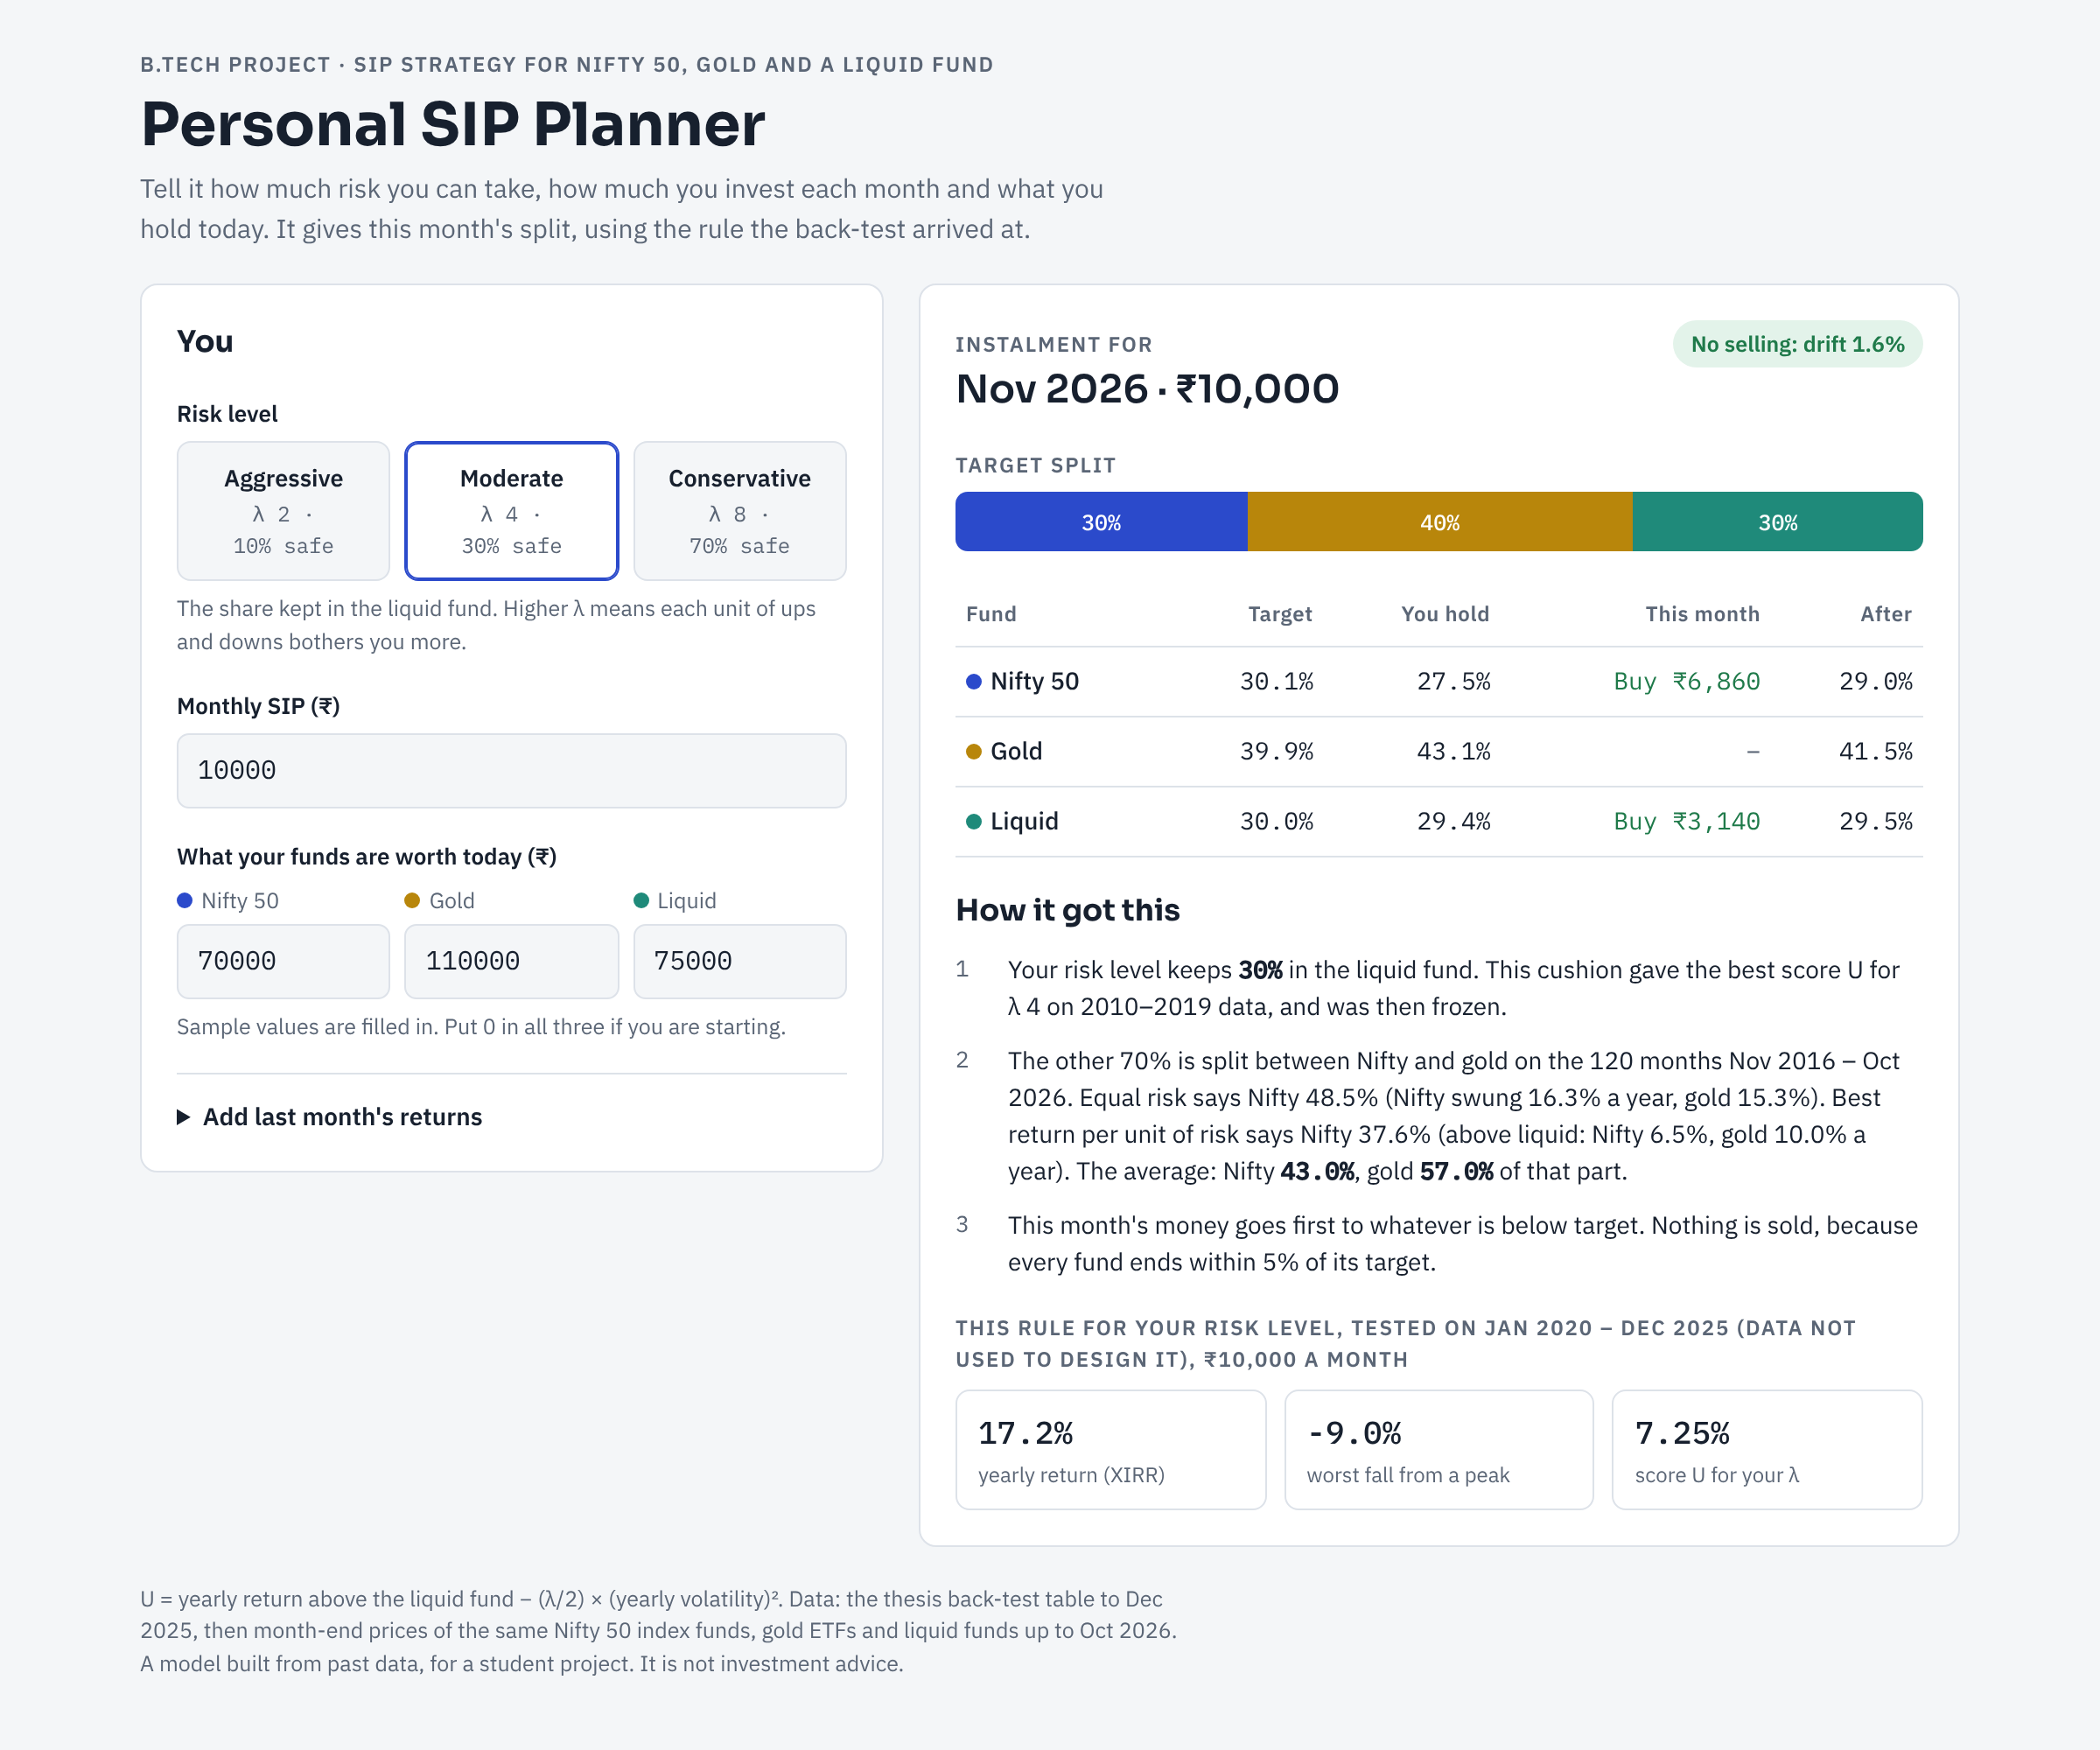
\includegraphics[width=\textwidth]{figures/website.png}
\caption{The planner for a moderate investor planning the November 2026 instalment}
\label{fig:website}
\end{figure}

\section{Design}

\begin{itemize}
  \item \textbf{Runs entirely in the browser.} The page carries the latest 120 months of returns,
        the frozen cushions and the 2020--2025 test results in a small data file (about 6~KB). All
        calculations run on the user's device; nothing the user types is sent anywhere. Months the
        user adds are stored only in their own browser.
  \item \textbf{Same rule as the back-test.} The engine (\code{sip.js}, Appendix~\ref{app:code}) is a
        JavaScript translation of the Python functions used in Chapters~\ref{ch:method}
        and~\ref{ch:results}: \code{optimized\_cash\_buffer} for the target and \code{\_smart\_split}
        with the 5\% band for the purchases.
  \item \textbf{Two-asset closed forms.} With only Nifty and gold in the risky part, risk parity
        uses Eq.~\eqref{eq:rp2} directly, and maximum Sharpe is found by evaluating 2{,}001 evenly
        spaced Nifty shares between the bounds and refining the best one by golden-section search.
  \item \textbf{Hosting.} The site is three static files (\code{index.html}, \code{sip.js},
        \code{data.js}) served free by GitHub Pages from a public repository.
\end{itemize}

\begin{figure}[H]
\centering
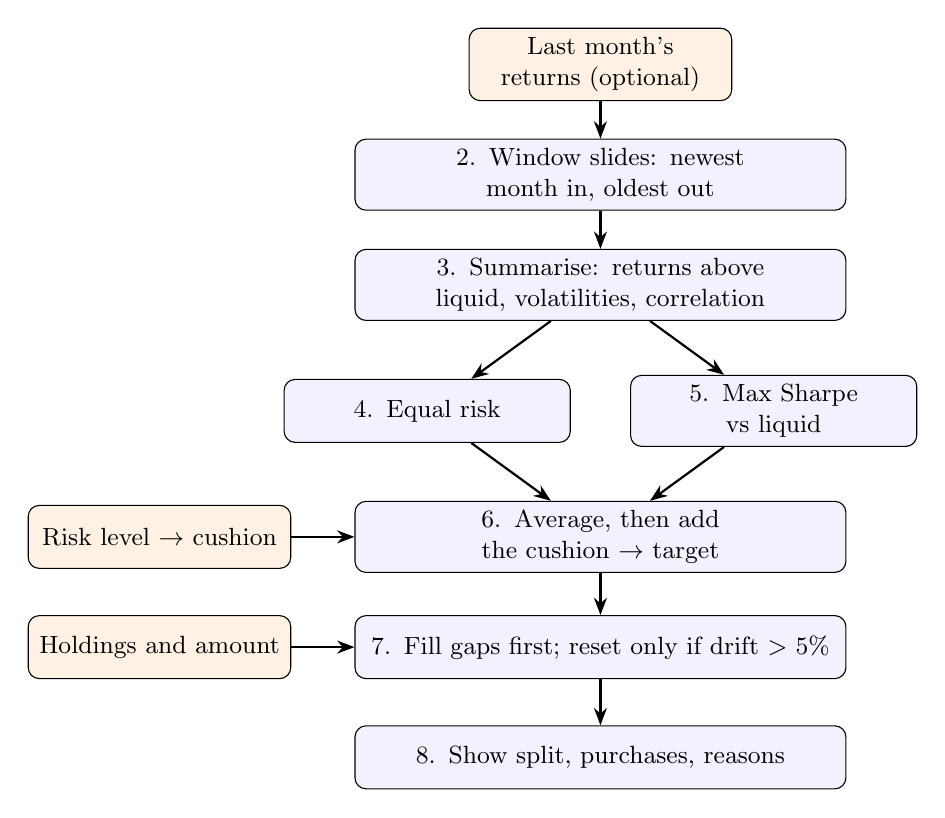
\begin{tikzpicture}[
  box/.style={draw, rounded corners, fill=blue!5, align=center, minimum height=8mm, text width=3.4cm, font=\small},
  wide/.style={box, text width=6cm},
  inp/.style={draw, rounded corners, fill=orange!10, align=center, minimum height=8mm, text width=3.1cm, font=\small},
  arr/.style={-{Stealth[length=2.2mm]}, thick}]
\node[inp]  (ret)  at (0,0)      {Last month's returns (optional)};
\node[wide] (s2)   at (0,-1.4)   {2. Window slides: newest month in, oldest out};
\node[wide] (s3)   at (0,-2.8)   {3. Summarise: returns above liquid, volatilities, correlation};
\node[box]  (s4)   at (-2.2,-4.4) {4. Equal risk};
\node[box]  (s5)   at (2.2,-4.4)  {5. Max Sharpe vs liquid};
\node[wide] (s6)   at (0,-6.0)   {6. Average, then add the cushion $\rightarrow$ target};
\node[inp]  (risk) at (-5.6,-6.0) {Risk level $\rightarrow$ cushion};
\node[wide] (s7)   at (0,-7.4)   {7. Fill gaps first; reset only if drift $> 5\%$};
\node[inp]  (hold) at (-5.6,-7.4) {Holdings and amount};
\node[wide] (s8)   at (0,-8.8)   {8. Show split, purchases, reasons};
\draw[arr] (ret) -- (s2); \draw[arr] (s2) -- (s3);
\draw[arr] (s3) -- (s4); \draw[arr] (s3) -- (s5);
\draw[arr] (s4) -- (s6); \draw[arr] (s5) -- (s6);
\draw[arr] (risk) -- (s6); \draw[arr] (s6) -- (s7); \draw[arr] (hold) -- (s7); \draw[arr] (s7) -- (s8);
\end{tikzpicture}
\caption{What the planner computes each time an input changes}
\label{fig:site-flow}
\end{figure}

\section{A complete worked example}
\label{sec:example}

This section follows the exact calculation behind Figure~\ref{fig:website}: a \textbf{moderate}
investor ($\lambda = 4$, cushion $L = 30\%$) on 1 November 2026, investing \Rs10{,}000 and holding
Nifty \Rs70{,}000, gold \Rs1{,}10{,}000 and liquid \Rs75{,}000. The window is the 120 months
November 2016 -- October 2026.

\subsection{Step 1: summarise the window}

\paragraph{Return above liquid.} For each month, the liquid return is subtracted from the Nifty and
gold returns; the 120 differences are averaged and multiplied by 12:
\begin{align*}
  \text{Nifty: }& 0.647872 / 120 = 0.005399 \text{ a month} \times 12 = 6.48\% \text{ a year},\\
  \text{Gold: }& 0.997018 / 120 = 0.008308 \text{ a month} \times 12 = 9.97\% \text{ a year}.
\end{align*}

\paragraph{Volatility.} The squared deviations from the mean are summed, divided by $n-1 = 119$, and
the square root is annualised with $\sqrt{12} = 3.464$:
\begin{align*}
  \text{Nifty: }& \sqrt{0.263199/119} = 4.703\% \text{ a month} \;\Rightarrow\; 16.29\% \text{ a year}
     \quad (V_N = 0.026541),\\
  \text{Gold: }& \sqrt{0.233427/119} = 4.429\% \text{ a month} \;\Rightarrow\; 15.34\% \text{ a year}
     \quad (V_G = 0.023539).
\end{align*}

\paragraph{Co-movement.} The products of the two assets' monthly deviations sum to $-0.0110126$;
divided by 119 and multiplied by 12, the yearly covariance is $C = -0.0011105$, and the correlation
is $-0.044$. Over this decade, Nifty and gold were practically unrelated.

\subsection{Step 2: bounds}

The risky part is $1 - L = 70\%$ of the money. Nifty and gold must each hold at least 10\% and at
most 70\% of the whole portfolio. For \Rs1{,}00{,}000 this means \Rs70{,}000 to split, of which each
must get at least \Rs10{,}000, so the Nifty share of the risky part lies between
$10{,}000/70{,}000 = 14.29\%$ and $60{,}000/70{,}000 = 85.71\%$.

\subsection{Step 3: equal risk}

From Eq.~\eqref{eq:rp2}:
\[
  n_{\text{RP}} = \frac{15.34}{16.29 + 15.34} = \frac{15.34}{31.63} = 48.50\% .
\]
Check with Eq.~\eqref{eq:rc}:
$RC_N = 0.4850\,(0.4850 \times 0.026541 + 0.5150 \times (-0.0011105)) = 0.005966$ and
$RC_G = 0.5150\,(0.5150 \times 0.023539 + 0.4850 \times (-0.0011105)) = 0.005966$.
Both assets contribute equally.

\subsection{Step 4: maximum Sharpe above liquid}

For a Nifty share $w$ of the risky part:
$m = 6.48\%\,w + 9.97\%\,(1-w)$, \;
$v = w^2 V_N + 2w(1-w)C + (1-w)^2 V_G$, \;
score $= m/\sqrt{v}$.

\begin{table}[H]
\centering
\caption{Some of the 2{,}001 mixes evaluated}
\label{tab:ms-search}
\begin{adjustbox}{max width=\textwidth}
\begin{tabular}{@{}rrrr@{}}
\toprule
Nifty share $w$ & Return above liquid $m$ & Volatility $\sqrt{v}$ & Score $m/\sqrt{v}$ \\
\midrule
14.29\% (lowest allowed) & 9.47\% & 13.25\% & 0.715 \\
30.00\% & 8.92\% & 11.60\% & 0.769 \\
\textbf{37.57\%} & \textbf{8.66\%} & \textbf{11.14\%} & \textbf{0.778} \\
50.00\% & 8.22\% & 10.94\% & 0.752 \\
70.00\% & 7.53\% & 12.11\% & 0.622 \\
85.71\% (highest allowed) & 6.98\% & 14.04\% & 0.497 \\
\bottomrule
\end{tabular}
\end{adjustbox}
\end{table}

At the best mix, $w = 0.3757$:
\begin{align*}
  m &= 0.3757 \times 6.48\% + 0.6243 \times 9.97\% = 8.66\%,\\
  v &= \underbrace{0.003746}_{w^2V_N} \; \underbrace{-\,0.000521}_{2w(1-w)C} \; + \underbrace{0.009174}_{(1-w)^2V_G} = 0.012400,
      \qquad \sqrt{v} = 11.14\%,\\
  \text{score} &= 8.66 / 11.14 = 0.778 .
\end{align*}
A 38/62 mix swings 11.1\% a year, less than Nifty (16.3\%) or gold (15.3\%) alone: the
diversification effect of Section~\ref{sec:maxsharpe}.

\subsection{Step 5: the target}

\[
  n = \tfrac12 \times 48.50\% + \tfrac12 \times 37.57\% = 43.03\%,
\]
\begin{align*}
  w_{\text{Nifty}} &= 0.70 \times 43.03\% = 30.12\%, \\
  w_{\text{Gold}} &= 0.70 \times 56.97\% = 39.88\%, \\
  w_{\text{Liquid}} &= 30.00\% .
\end{align*}

\subsection{Step 6: this month's purchases}

The total after investing is $70{,}000 + 1{,}10{,}000 + 75{,}000 + 10{,}000 = \Rs2{,}65{,}000$.

\begin{table}[H]
\centering
\caption{The smart split for the example investor}
\label{tab:example-split}
\begin{adjustbox}{max width=\textwidth}
\begin{tabular}{@{}lrrrrr@{}}
\toprule
Fund & Target & Should hold & Holds now & Gap & Buy \\
\midrule
Nifty & 30.12\% & \Rs79{,}830 & \Rs70{,}000 & \Rs9{,}830 & \Rs6{,}860 \\
Gold & 39.88\% & \Rs1{,}05{,}670 & \Rs1{,}10{,}000 & 0 & 0 \\
Liquid & 30.00\% & \Rs79{,}500 & \Rs75{,}000 & \Rs4{,}500 & \Rs3{,}140 \\
\midrule
Total & & & & \Rs14{,}330 & \Rs10{,}000 \\
\bottomrule
\end{tabular}
\end{adjustbox}
\end{table}

The gaps exceed the instalment, so by Eq.~\eqref{eq:smart} the money is shared in proportion:
$9{,}830/14{,}330 \times 10{,}000 = \Rs6{,}860$ to Nifty and
$4{,}500/14{,}330 \times 10{,}000 = \Rs3{,}140$ to liquid. Afterwards the shares are 29.0\%, 41.5\%
and 29.5\%. The largest drift is gold's 1.6 percentage points, below the 5\% band, so nothing is
sold. These are exactly the figures in Figure~\ref{fig:website}.

\section{Stability of the target}

A natural question is how much one unusual month changes the advice. As a test, an extreme month
was entered for November 2026: Nifty $+1\%$, gold $+20\%$, liquid $+10\%$.

\begin{table}[H]
\centering
\caption{Effect of extreme new months on the moderate investor's target}
\label{tab:stability}
\small
\begin{adjustbox}{max width=\textwidth}
\begin{tabular}{@{}lcccc@{}}
\toprule
Scenario & Equal risk & Max Sharpe & Average & Nifty / Gold / Liquid \\
\midrule
Window to Oct 2026 (as above) & 48.50\% & 37.57\% & 43.03\% & 30.1 / 39.9 / 30 \\
Add Nov: Nifty $+1\%$, gold $+20\%$, liquid $+10\%$ & 50.16\% & 36.45\% & 43.31\% & 30.3 / 39.7 / 30 \\
Add Nov: gold $+60\%$ & 59.68\% & 49.21\% & 54.45\% & 38.1 / 31.9 / 30 \\
Gold $+20\%$ every month for a year & 60.58\% & 30.93\% & 45.76\% & 32.0 / 38.0 / 30 \\
\bottomrule
\end{tabular}
\end{adjustbox}
\end{table}

The 20\% gold month moved the Nifty target by only 0.2 percentage points, for three reasons. It is
one month out of 120. The two advisers react in opposite directions: gold's higher average return
pulls maximum Sharpe towards gold, while gold's higher volatility pushes risk parity away from it.
And the liquid share is the fixed cushion, so the liquid fund's 10\% month cannot change it. Only a
shock large enough to raise gold's volatility sharply (the $+60\%$ case) moves both advisers the
same way. This stability is deliberate: the rule does not chase short-term spikes, which the
estimation-error literature suggests would be costly. The price is that it adapts slowly to a
genuine, lasting change.

\section{Verification}

\begin{itemize}
  \item An automated test runs \code{sip.js} under Node.js on the same 120-month window as the Python
        engine and requires the targets to agree within $10^{-6}$ and the rupee purchases within
        \Rs0.50, for all three profiles. The observed differences were below $10^{-8}$ for the
        targets and \Rs0.003 for the purchases.
  \item A second test checks that the page's data file is exactly the latest 120 months of the
        project's return table.
  \item The page was checked at desktop and phone widths and in light and dark themes.
\end{itemize}

\section{Limitations of the planner}

\begin{itemize}
  \item The risk level is chosen from three fixed profiles rather than measured by a questionnaire.
  \item Taxes and exit loads are not considered when recommending a sale.
  \item The data must be kept current: either the maintainer updates the data file, or the user adds
        each month's returns on the page.
  \item The planner is an educational output of a back-test, not investment advice.
\end{itemize}

\section{Conclusion and Future Work}
\label{ch:conclusion}

\subsection{Conclusions}

This project built a walk-forward back-testing engine for monthly SIPs in Nifty~50, gold and a
liquid fund, applied it to Indian data from 2000 to 2026, and turned the final rule into a public
planning tool. The main conclusions are:

\begin{enumerate}
  \item \textbf{Diversification across these three assets works.} Their correlations were low or
        negative throughout, and in every stress period studied the mixes lost far less than equity
        alone.
  \item \textbf{The risk-free benchmark matters.} With a cash-like liquid fund available, optimisers
        that measure risk against 0\% simply hold cash. Measuring returns above the liquid fund and
        treating it as cash, following \citet{tobin1958} and \citet{sharpe1994}, raised the
        optimised SIP's out-of-sample return from 11.1\% to 20.3\% a year.
  \item \textbf{Estimation error dominates.} The strategy that directly maximised the investor's
        utility never achieved the highest utility. Rules that depend less on estimated average
        returns, such as equal weights, fixed mixes and the risk-parity blend, held up better, in
        line with \citet{michaud1989}, \citet{chopra1993} and \citet{demiguel2009}.
  \item \textbf{The best strategy depends on the investor and the period.} Measured by utility, the
        ranking changed with risk aversion in 2010--2019 and with the gold boom in 2020--2025. No
        rule should be presented as universally best.
  \item \textbf{A personal cushion makes the advice personal.} The Personal SIP gives a conservative
        investor a much smaller worst fall ($-3.4\%$ against $-12.2\%$), at the cost of lower
        returns in strong markets. Its cushions, chosen on 2010--2019, proved too cautious for
        2020--2025.
  \item \textbf{The rule can be used in practice.} The planner turns the back-tested rule into a
        two-minute monthly routine, with results verified against the research code.
\end{enumerate}

\subsection{Limitations and future work}

The data before 2020 uses a constant 1.3\% Nifty dividend yield, international gold without Indian
import duty, and a T-bill index rather than a real liquid fund. The test period is only six years.
The values $\lambda = 2, 4, 8$ are assumed rather than measured, variance penalises gains as much as
losses, and taxes and exit loads are ignored. Natural extensions are: setting $\lambda$ from a risk
questionnaire; adding a drawdown penalty to $U$; shrinking estimated returns to reduce estimation
error; fetching fund prices automatically each month; and including taxes when deciding whether to
rebalance.


\bibliographystyle{plainnat}
\bibliography{references}


\end{document}
